
%(BEGIN_QUESTION)
% Copyright 2007, Tony R. Kuphaldt, released under the Creative Commons Attribution License (v 1.0)
% This means you may do almost anything with this work of mine, so long as you give me proper credit

Set up peer-to-peer EIA/TIA-232 networking between two personal computers, using the 9-pin male serial port connectors on the back.  You will need a {\it null modem} cable to connect the two computers, and each computer will need to run a {\it terminal emulator} program such as {\tt hyperterminal} or {\tt kermit}.

You may construct your own null modem cable using two 9-pin serial (DE-9) female connectors and cable wires connected like this:

$$\includegraphics[width=15.5cm]{i02211x01.eps}$$

Or, of you're feeling lazy, omit all the connections shown above except for the three wires between pins 2, 3, and 5.  Then, of course, you will have to set up the terminal emulator program for software handshaking instead of hardware handshaking.

\vskip 10pt

After setting up both terminal emulators for the same parameters (stop and data bits, parity, baud rate, etc.) and connecting the null modem cable, you should be able to type messages in one computer and read those messages on the other!

Try experimenting with different baud rates to see how fast you can send messages without errors!

\underbar{file i02211}
%(END_QUESTION)





%(BEGIN_ANSWER)

No answers provided here.  You'll have to try it yourself on a real computer!

%(END_ANSWER)





%(BEGIN_NOTES)

\vfil \eject

\noindent
{\bf Summary Quiz:}

(The recommended summary quiz is to have students demonstrate peer-to-peer text messaging between personal computers)

%INDEX% Networking, practical exercise: peer-to-peer EIA/TIA-232 network

%(END_NOTES)


